
\begin{figure}[!htbp]
\begin{centering}
                            % trim=left bottom right top
    {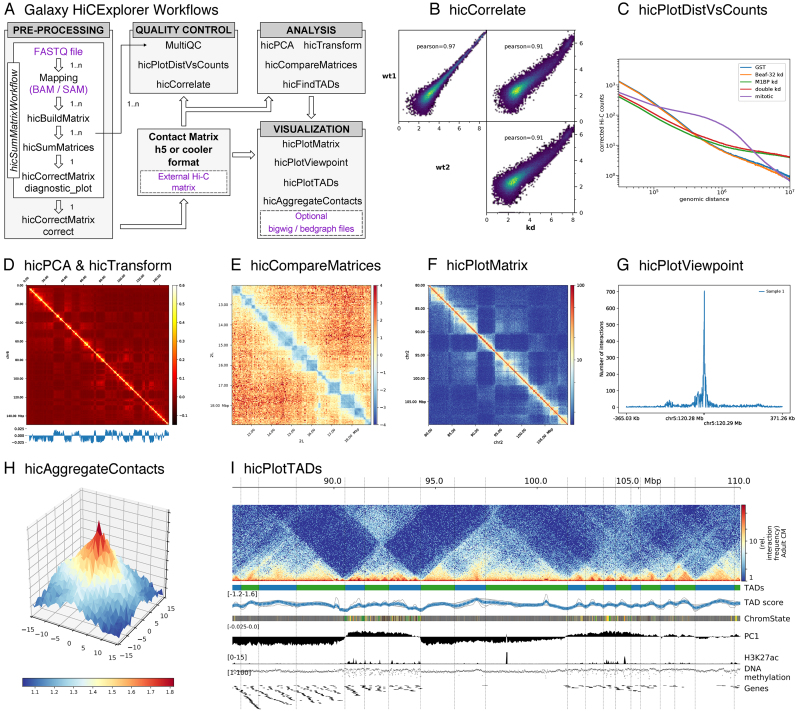
\includegraphics[scale=3.8,trim=37 0 0 45,clip]{figures/background/HiCExplorer.jpg}}
    \caption[Excerpt of HiCExplorer visualizations]
    {
        \textbf{Excerpt of HiCExplorer visualizations}
        \textbf{E)} Pixel difference computed using hicCompareMatrices and
        visualized using hicPlotMatrix of a Hi-C corrected matrix for wild type
        condition and knock down.
        \textbf{F)} Plot of a 80 to 105 Mb region contact matrix of chromosome 2 in log scale.
        \textbf{G)} Corrected number of Hi-C contacts shown using
        hicPlotViewpoint, for a single bin in chromosome 5 (output similar to
        4C-seq).
        \textbf{I)} Human chromosome 2 visualization (region 85-110 Mb) using
        tracks from different tools found in the HiCExplorer toolbox (primarily
        TAD-related information). \\
        \\Image adapted from \cite{wolff2018galaxy}.}
    \label{fig:comparison3C}\label{fig:HiCExplorer}
\end{centering}
\end{figure}



